% !TEX program = pdflatex
\documentclass[11pt,a4paper]{article}

% --- packages ---
\usepackage[utf8]{inputenc}
\usepackage[T1]{fontenc}
\usepackage{lmodern}
\usepackage{geometry}
\geometry{margin=1in}
\usepackage{amsmath,amssymb}
\usepackage{siunitx}
\usepackage{graphicx}
\usepackage[font=small,labelfont=bf,labelsep=endash]{caption}
\usepackage{booktabs}
\usepackage{physics}
\usepackage{hyperref}
\hypersetup{colorlinks=true,linkcolor=blue,citecolor=blue,urlcolor=blue}

% --- title & author ---
\title{Design Methodology for a Dual-Jet Hovering Disc with Concentric Air Curtains:\\
Model, Non-Dimensionalization, and Simulation Outputs}
\author{ }
\date{ }

\begin{document}
\maketitle

\begin{abstract}
We present a modeling and design framework for a hovering disc sustained by two concentric air jets: an outer annular jet (air curtain) that confines the inner flow and reduces leakage, and an inner make-up jet that maintains the cushion overpressure.
The analysis adopts a low-Mach compressible, axisymmetric core model with an anisotropic Stokes--Darcy closure and avoids thin-film assumptions ($h\sim R_{\mathrm{tot}}$). We state the lift and leakage balances, the curtain momentum condition, and a computational algorithm.
A \emph{non-dimensionalization strategy} is provided so that the accompanying Python tool produces parameter-agnostic plots. This document also loads the simulation figures saved by the script into the repository's shared \texttt{../figs/} directory, keeping a stable linkage between code and paper.
\end{abstract}

\section{Geometry and Notation}
We use the schematic in Fig.~\ref{fig:geometry} and the following notation:
\begin{itemize}
  \item $R_{\mathrm{tot}}$ total radius; $w$ leakage-ring width; $R^{-}=R_{\mathrm{tot}}-w$ inner edge of the peripheral ring;
  \item $h$ disc--ground clearance; $h_{\mathrm{eff}}$ effective sealing height at the rim; $b$ slot thickness of the curtain;
  \item $W$ payload; $p_0$ ambient pressure; $p_c=W/(\pi R_{\mathrm{tot}}^2)$ cushion overpressure;
  \item Outer jet (\emph{corona}): exit speed $U_{\mathrm{corona}}$, jet density $\rho_j$, slot area $A_{\mathrm{corona}}=2\pi R_{\mathrm{tot}}\,b$;
  \item Inner jet: mass flow $\dot m_{\mathrm{in}}$; leakage $\dot m_{\mathrm{loss}}$; volumetric loss $Q_{\mathrm{loss}}=\dot m_{\mathrm{loss}}/\rho_{\mathrm{edge}}$.
\end{itemize}

\begin{figure}[t]
  \centering
  % All figures are loaded from the common ../figs/ directory
  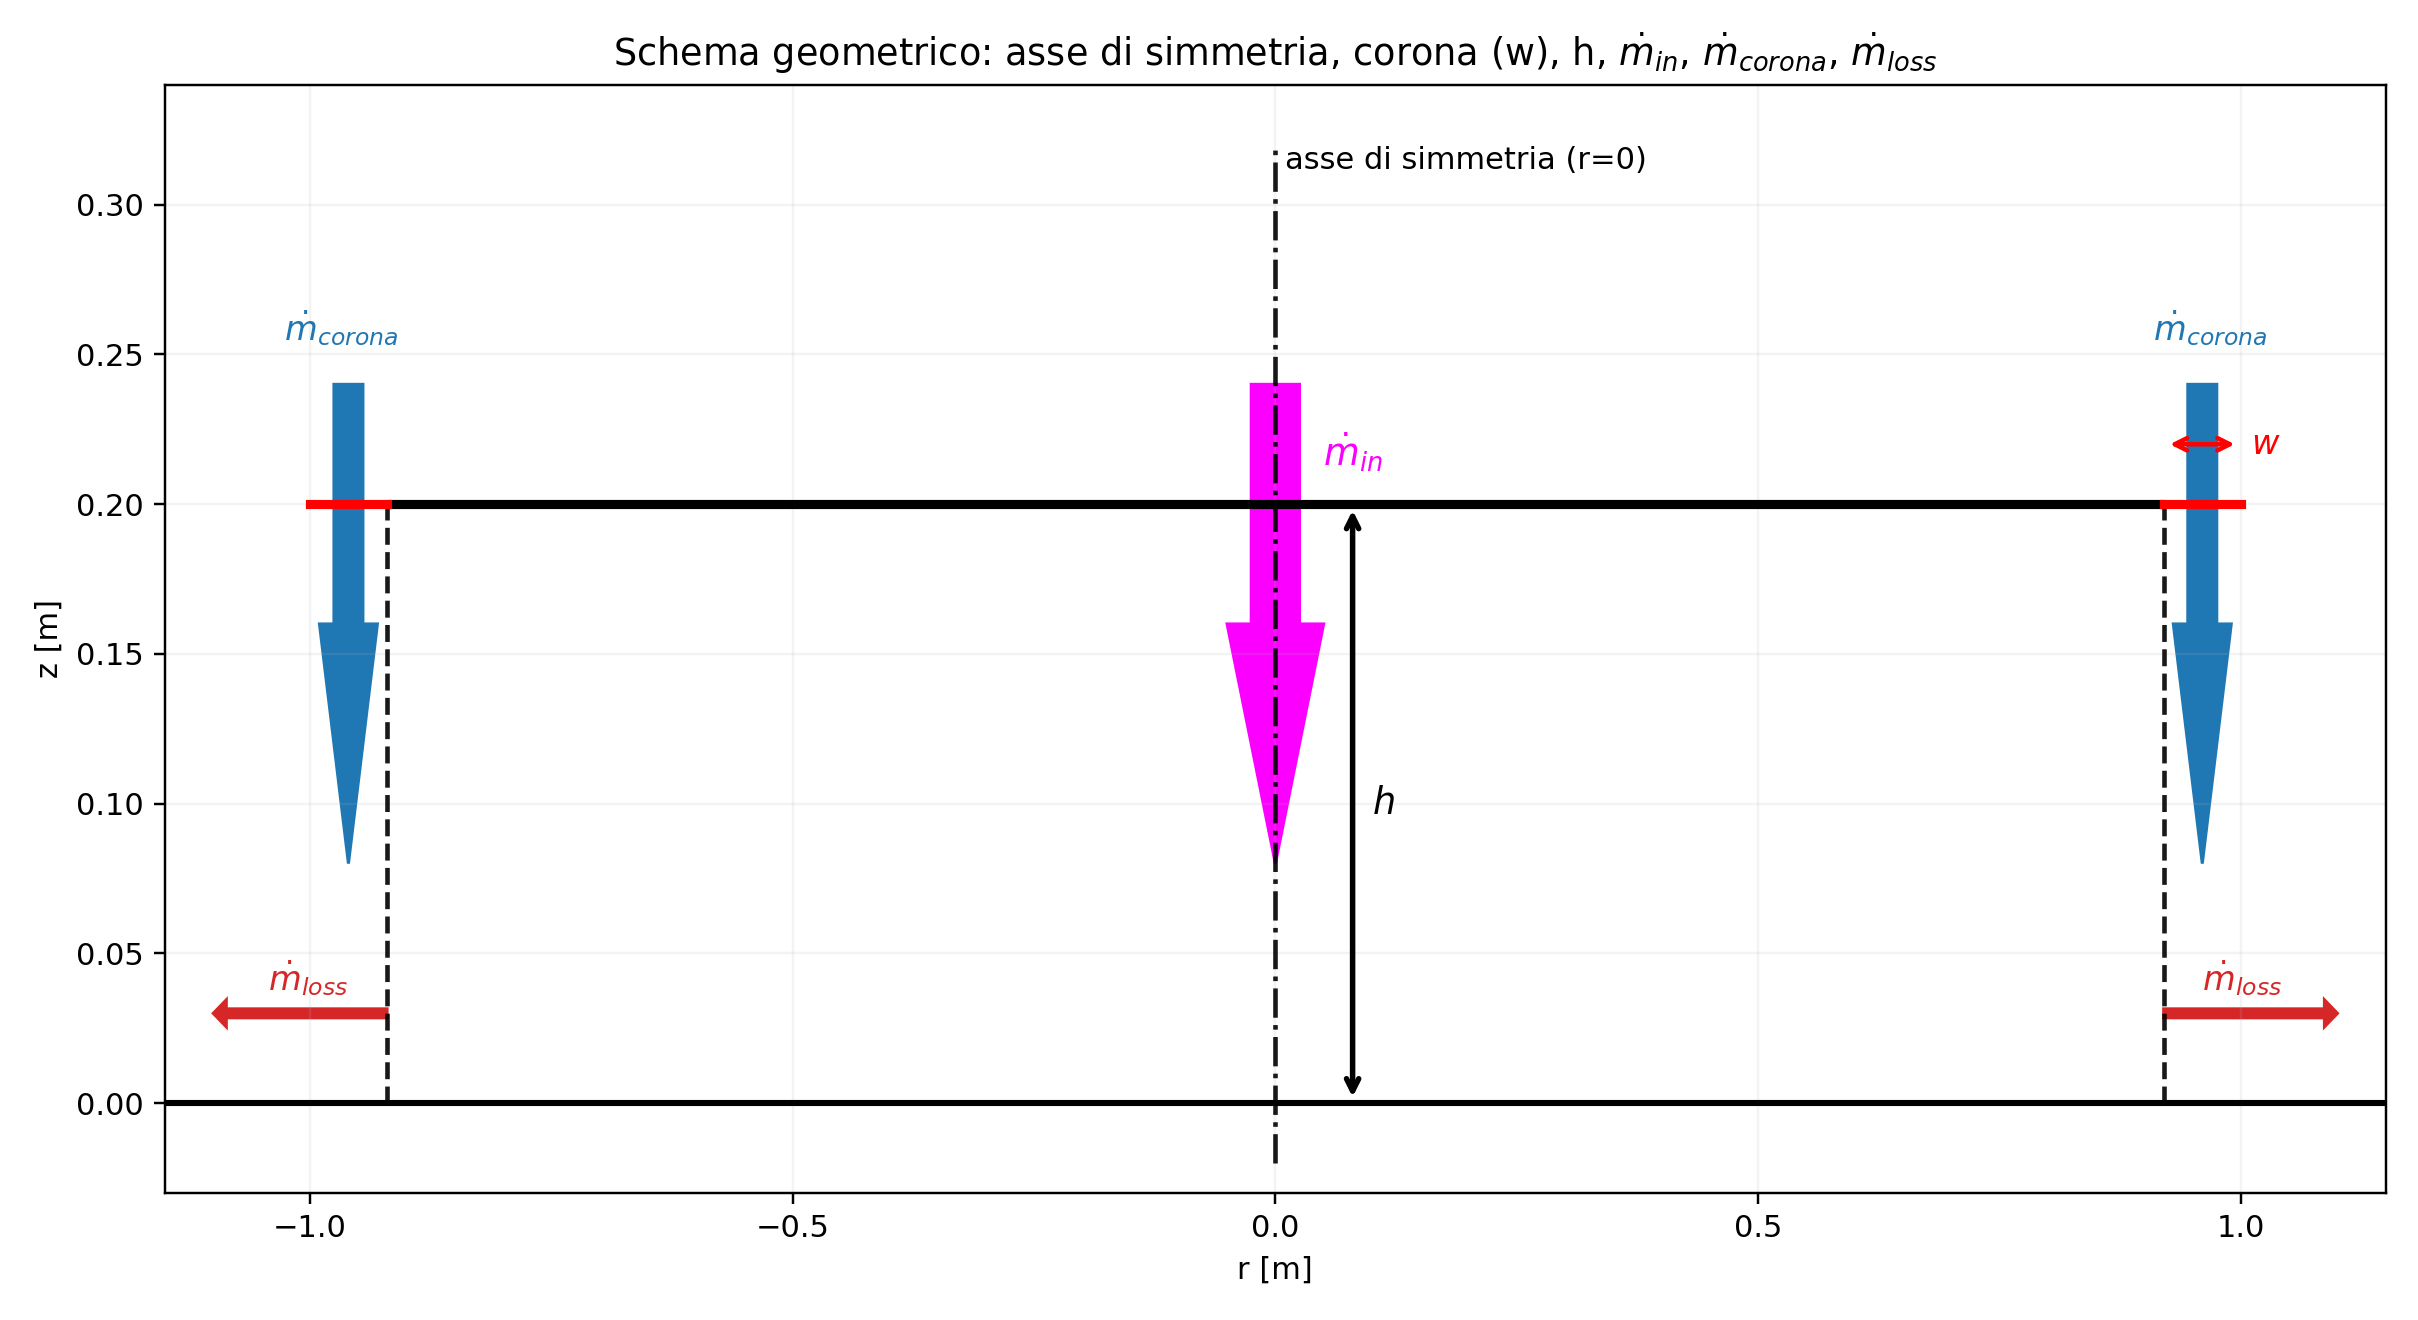
\includegraphics[width=0.95\linewidth]{../figs/schema_geometry.png}
  \caption{Geometry and notation. The domain for the core model is $(r,z)\in[0,R^{-}]\times[0,h]$; the outer annular jet issues vertically downward at $z=h$ on $R^{-}\le r\le R_{\mathrm{tot}}$, then turns near the floor forming a sealing curtain.}
  \label{fig:geometry}
\end{figure}

\section{Core Model and Sealing Condition (summary)}
We adopt the anisotropic Stokes--Darcy closure for mean velocities
\begin{equation}
  u = -\frac{\kappa_r}{\mu}\,\partial_r p,\qquad
  w = -\frac{\kappa_z}{\mu}\,\partial_z p,\qquad
  \kappa_r=\alpha_r h^2,\ \kappa_z=\alpha_z h^2,
\end{equation}
with compressible continuity and ideal-gas state $p=\rho R_g T$.
The design-oriented pressure equation in the core reads
\begin{equation}
  \frac{1}{r}\,\partial_r\!\big(r\,\rho\,\kappa_r\,\partial_r p\big)+\partial_z\!\big(\rho\,\kappa_z\,\partial_z p\big)=0,
\end{equation}
with BCs: symmetry at $r=0$; no-normal-flow at $z=0$ and $z=h$; and a \emph{rim pressure} at $r=R^{-}$ induced by the turned curtain,
\begin{equation}
  p_{\mathrm{edge}}(z)=p_0 + \Delta p\,\Phi\!\left(\frac{z}{h}\right),\qquad
  \Delta p = C_t\,\frac{\rho_j U_{\mathrm{corona}}^2\,b}{h_{\mathrm{eff}}}.
\end{equation}
To ensure a downward vertical component in the core ($w<0$), one convenient choice is an \emph{increasing} profile $\Phi(\zeta)$ so that $\partial_z p>0$ and $w=-(\kappa_z/\mu)\partial_z p<0$.

\section{Non-Dimensionalization and Plotting Conventions}
We scale
\begin{equation}
  \hat r=\frac{r}{R_{\mathrm{tot}}},\quad
  \hat z=\frac{z}{h},\quad
  \hat p=\frac{p-p_0}{p_c},\quad
  \hat T=\frac{T}{T_\infty},\quad
  \hat\rho=\frac{\rho}{\rho_\infty}=\frac{1+\Pi_p\,\hat p}{\hat T},\ \ \Pi_p=\frac{p_c}{p_0}.
\end{equation}
The non-dimensional elliptic equation is
\begin{equation}
  \frac{1}{\hat r}\,\partial_{\hat r}\!\big(\hat r\,\hat\rho\,\partial_{\hat r}\hat p\big)
  + \mathcal{A}\,\partial_{\hat z}\!\big(\hat\rho\,\partial_{\hat z}\hat p\big)=0,\qquad
  \mathcal{A}=\frac{\alpha_z}{\alpha_r}\left(\frac{R_{\mathrm{tot}}}{h}\right)^2,
\end{equation}
with BCs $\partial_{\hat r}\hat p(0,\hat z)=0$, $\partial_{\hat z}\hat p(\hat r,0)=\partial_{\hat z}\hat p(\hat r,1)=0$, and
$\hat p(\hat R^{-},\hat z)=\Pi_{\mathrm{edge}}\Phi(\hat z)$, where $\hat R^{-}=R^{-}/R_{\mathrm{tot}}$ and
\begin{equation}
  \Pi_{\mathrm{edge}}=\frac{p_{\mathrm{edge}}-p_0}{p_c}=\frac{C_t\,\rho_j U_{\mathrm{corona}}^2\,b}{h_{\mathrm{eff}}\,p_c}.
\end{equation}
Natural velocity scales are
\begin{equation}
  U_r^0=\frac{\kappa_r}{\mu}\,\frac{p_c}{R_{\mathrm{tot}}},\qquad
  U_z^0=\frac{\kappa_z}{\mu}\,\frac{p_c}{h},\qquad
  S=\frac{U_z^0}{U_r^0}=\frac{\alpha_z}{\alpha_r}\frac{R_{\mathrm{tot}}}{h}.
\end{equation}
The dimensionless velocities for plotting are
\begin{equation}
  \hat u=-\partial_{\hat r}\hat p,\qquad
  \hat w=-\partial_{\hat z}\hat p,\qquad
  \hat V_{\mathrm{iso}}=\sqrt{\hat u^{\,2}+S^{2}\hat w^{\,2}}.
\end{equation}

\section{Simulation Outputs (loaded from \texttt{../figs/})}
The Python script \texttt{scripts/run\_sim.py} solves the core problem and \emph{exports non-dimensional plots} to the shared directory \texttt{../figs/} with the filenames referenced below. Each figure uses axes $(\hat r,\hat z)$ and draws a vertical reference at $\hat r=\hat R^{-}$.
\begin{figure}[t]
  \centering
  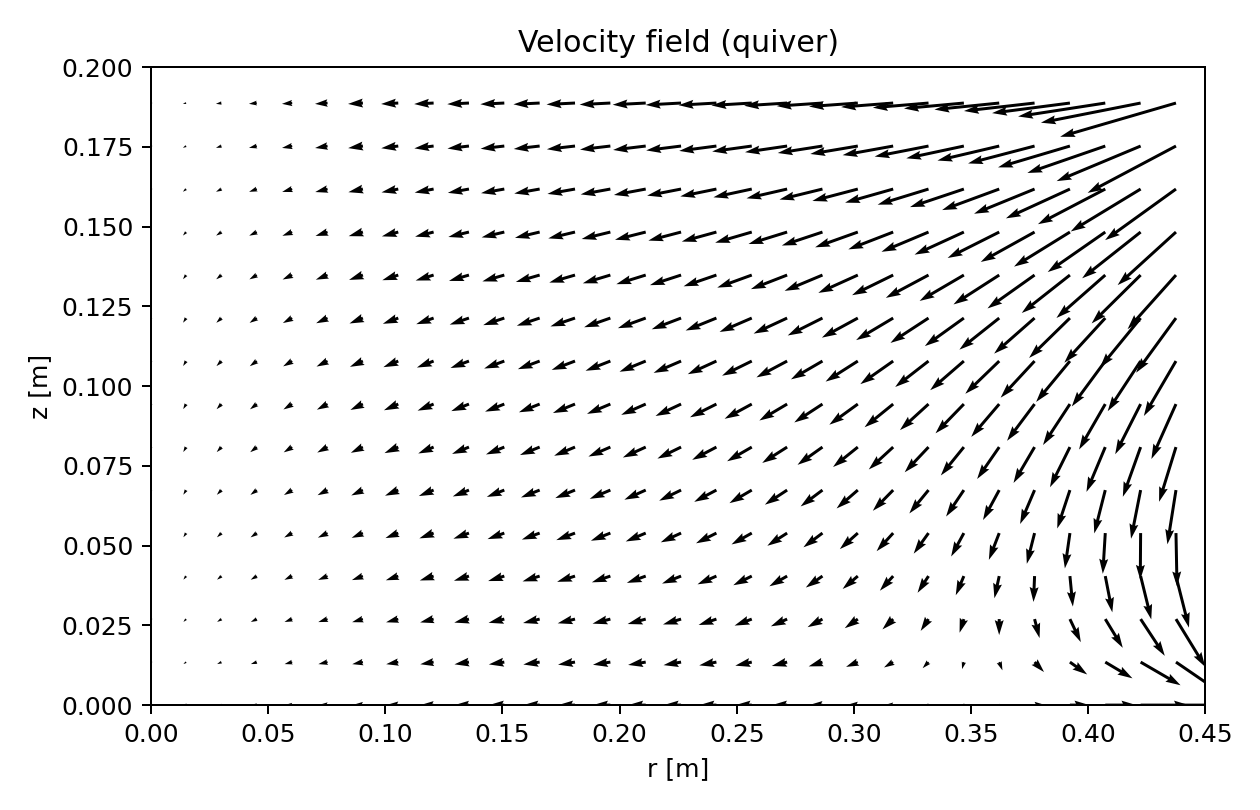
\includegraphics[width=0.95\linewidth]{../figs/quiver_velocity.png}
  \caption{Non-dimensional velocity field (quiver). Vectors show $(\hat u,\,S\hat w)$ for isotropic visual scaling; downward components reflect the vertical-jet condition at $z=h$.}
  \label{fig:quiver}
\end{figure}

\begin{figure}[t]
  \centering
  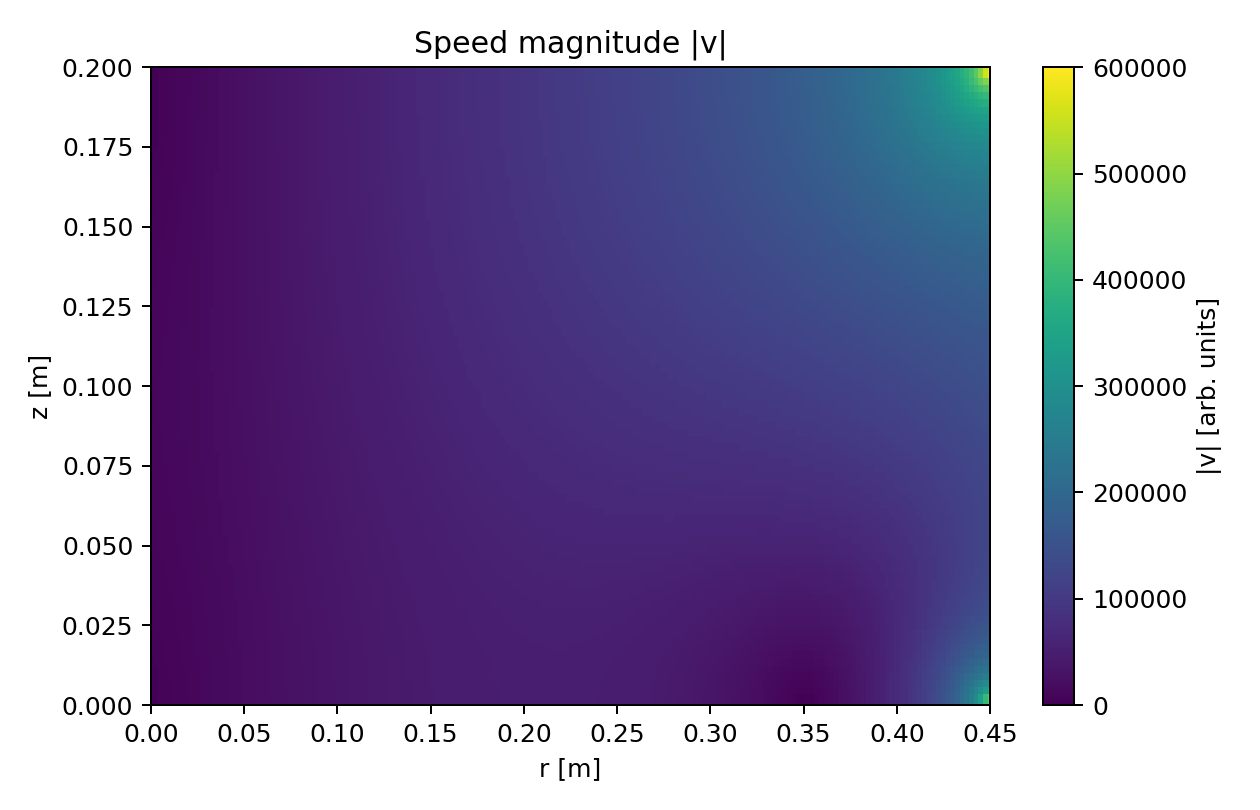
\includegraphics[width=0.95\linewidth]{../figs/cmap_speed.png}
  \caption{Colormap of the non-dimensional isotropic speed magnitude $\hat V_{\mathrm{iso}}=\sqrt{\hat u^{\,2}+S^{2}\hat w^{\,2}}$.}
  \label{fig:cmap_speed}
\end{figure}

\begin{figure}[t]
  \centering
  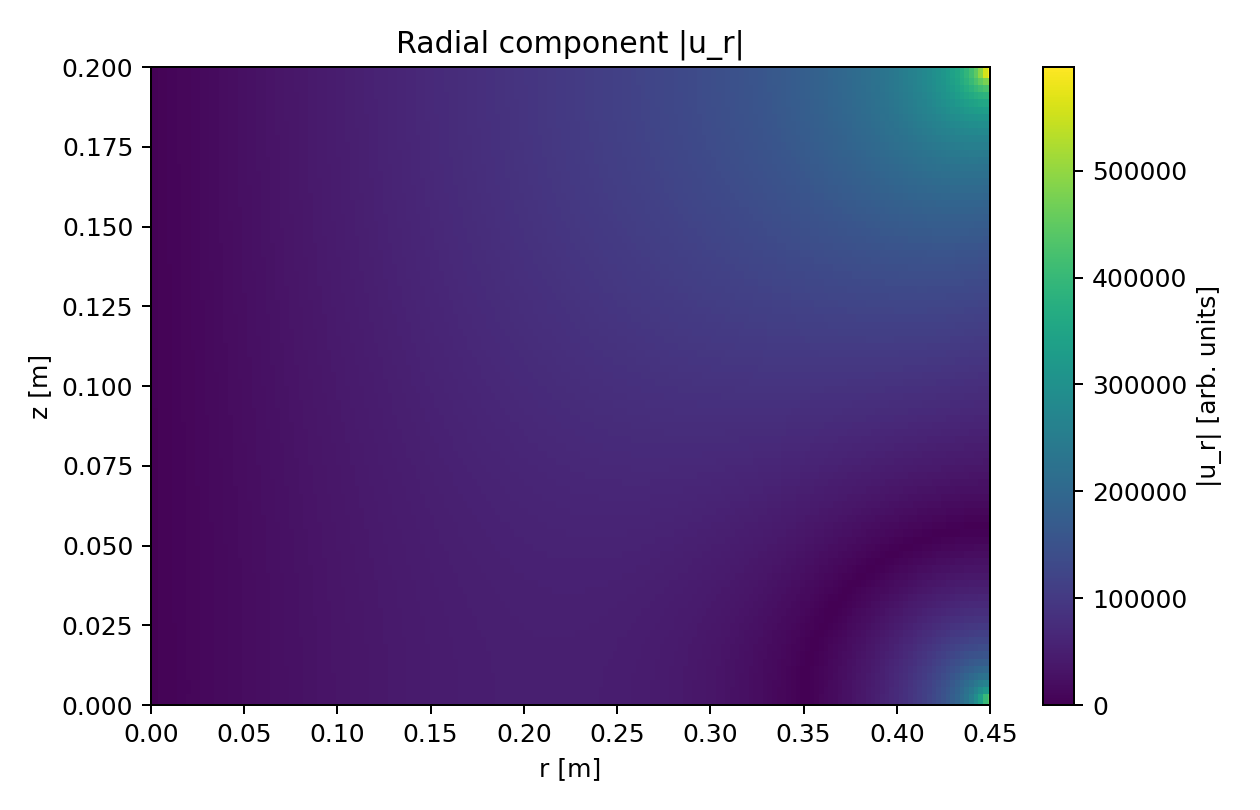
\includegraphics[width=0.95\linewidth]{../figs/cmap_ur.png}
  \caption{Colormap of the non-dimensional radial component magnitude $|\hat u|$.}
  \label{fig:cmap_ur}
\end{figure}

\begin{figure}[t]
  \centering
  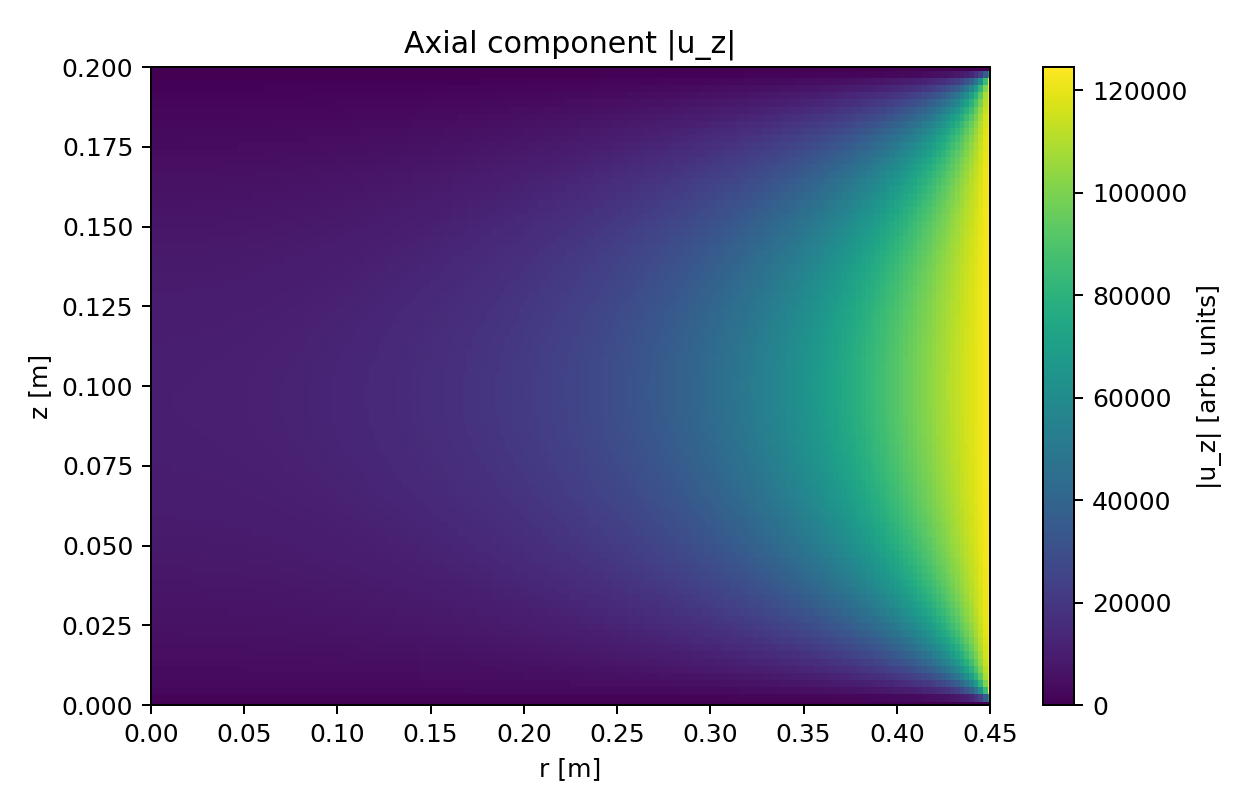
\includegraphics[width=0.95\linewidth]{../figs/cmap_uz.png}
  \caption{Colormap of the non-dimensional axial component magnitude $|\hat w|$.}
  \label{fig:cmap_uz}
\end{figure}

\begin{figure}[t]
  \centering
  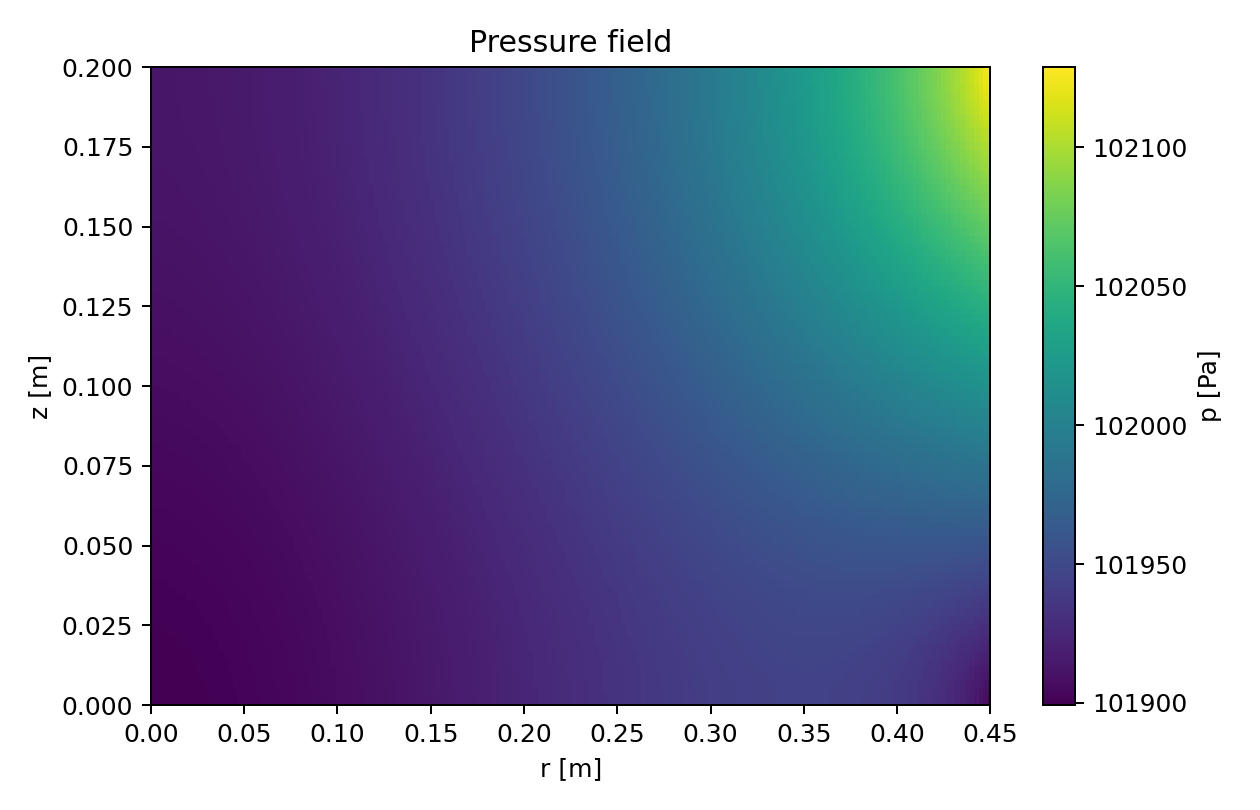
\includegraphics[width=0.95\linewidth]{../figs/cmap_pressure.png}
  \caption{Colormap of the non-dimensional pressure $\hat p$.}
  \label{fig:cmap_p}
\end{figure}

\end{document}
